%% Classe du document
\documentclass[a4paper,10pt]{article}

%% Francisation
\usepackage[francais]{babel} % Indique que l'on utilise le francais
\usepackage[T1]{fontenc}
\usepackage[utf8]{inputenc} % Indique que l'on utilise tout le clavier
%\usepackage[latin1]{inputenc}

%% Réglages généraux
\usepackage[top=3cm, bottom=3cm, left=3cm, right=3cm]{geometry} % Taille de la feuille
\usepackage{lastpage}

%% Package pour le texte
\usepackage{soul} % Souligner
\usepackage{color} % Utilisation de couleurs
\usepackage{hyperref} % Créer des liens et des signets
\usepackage{eurosym}% Pour le symbole euro
\usepackage{fancyhdr}% Entête et pied de page

%% Package pour les tableaux
\usepackage{multirow} % Colonnes multiples
\usepackage{cellspace}
\usepackage{array}

%% Package pour les dessins
\usepackage{pstricks}
\usepackage{graphicx} % Importer des images
\usepackage{pdftricks} % Pour utiliser avec pdfTex
\usepackage{pst-pdf} % Pour utiliser avec pdfTex
\usepackage{pst-node} % Pose de noeuds
\usepackage{subfig}
\usepackage{float}

%% Package pour les maths
\usepackage{amsmath} % Commandes essentielles
\usepackage{amssymb} % Principaux symboles

%% Package pour le code
\usepackage{listings} % Utilisation de la couleur syntaxique des langages
\usepackage{url}


\usepackage[babel=true]{csquotes} % Permet les quotations (guillemets)
\usepackage{tocvsec2}
\usepackage{amsthm}
\usepackage{amsfonts}

\usepackage{tikz}
\usepackage{pdfpages}

\usetikzlibrary{shapes} % A revoir

%--------------------- Autres définitions ---------------------%

% Propriété des liens
\hypersetup{
colorlinks = true, % Colorise les liens
urlcolor = blue, % Couleur des hyperliens
linkcolor = black, % Couleur des liens internes
}

\definecolor{grey}{rgb}{0.95,0.95,0.95}

% Language Definitions for Turtle
%TODO: a revoir avec les couleur de gedit
\definecolor{olivegreen}{rgb}{0.2,0.8,0.5}
\definecolor{grey2}{rgb}{0.5,0.5,0.5}
\lstdefinelanguage{ttl}{
sensitive=true,
morecomment=[s][\color{grey2}]{@}{:},
morecomment=[l][\color{olivegreen}]{\#},
morecomment=[s][\color{red}]{<}{/>},
morestring=[s][\color{olivegreen}]{<http://w}{\#>},
morestring=[b][\color{blue}]{\"},
}

\lstset{
frame=single,
breaklines=true,
basicstyle=\ttfamily,
backgroundcolor=\color{grey},
basicstyle=\scriptsize,
keywordstyle=\color{blue},
commentstyle=\color{green},
stringstyle=\color{red},
identifierstyle=\color{blue}
}

%Definition de la commande pour retirer l'espace devant les ':'
\makeatletter
\@ifpackageloaded{babel}%
        {\newcommand{\nospace}[1]{{\NoAutoSpaceBeforeFDP{}#1}}}%  % !! double {{}} pour cantonner l'effet à l'argument #1 !!
        {\newcommand{\nospace}[1]{#1}}
\makeatother

\setcounter{tocdepth}{3}
%\maxsecnumdepth{subsubsection} % Dernière section numérotée

\newcommand{\paperPrototyping}{\emph{paper prototyping}}

% Corps du document :
\begin{document}

% Définition des entêtes et pieds de page
\fancyhead[LE,CE,RE,LO,CO,RO]{}
\fancyfoot[LE,CE,RE,LO,CO,RO]{}
\fancyhead[LO, LE]{English}
\fancyhead[RO,RE]{2012/2013}
\fancyfoot[LO,LE]{Université de \scshape{Nantes}}
\fancyfoot[RO,RE]{Page \thepage \ sur \pageref{LastPage}}
\renewcommand{\headrulewidth}{0.4pt}
\renewcommand{\footrulewidth}{0.4pt}

%\maketitle
\begin{titlepage}

\vspace*{\fill}~
\begin{center}
{\large \textsc{Guide}} \\
\vspace{1cm}
{\LARGE How to create a beautiful blog} \\
\vspace{1cm}
COUTABLLE Guillaume, MENORET Clément, RULLIER Noémie, WOLLENBURGER Antoine \\
\today
\end{center}
\vspace*{\fill}

\vspace{\stretch{1}}
\begin{center}
\noindent 

\includegraphics[height=2.5cm]{Images/universite.png}
\end{center}
\pagebreak
\end{titlepage}

\newpage
\tableofcontents 

% Introduction
\newpage
\pagestyle{fancy}

%TODO : Correction des fautes d'orthographes, tournures de phrases ...
%TODO : En fonction des parties de tous le monde redire à Nomyx de diminuer ses images pour pas que ça dépasse 10 page (environ)
%TODO : Je ne sais pas si c'est address email ou email address --> J'ai utiliser les deux sens donc à revoir

%%%%%%%%%%%%%%%%%%%%%%%%%%%%%%%%%%%%%%%%%%%%%%%%%%%%%%%%%%%%%%%%%%%%%%%%%%%%%
%%%%%%%%%%  Introduction générale
%%%%%%%%%%%%%%%%%%%%%%%%%%%%%%%%%%%%%%%%%%%%%%%%%%%%%%%%%%%%%%%%%%%%%%%%%%%%%
\section{Introduction}
There are a lots of tools available to create a blog. There are intended to different persons from novice to professional.

This document is a tutorial to help you to create your own blog. We consider that you are not a expert, that's why we choose a tool adapt to all public. We will work with \emph{Overblog}.

To realise this tutorial, you need a internet connection and a valide email address.

%%%%%%%%%%%%%%%%%%%%%%%%%%%%%%%%%%%%%%%%%%%%%%%%%%%%%%%%%%%%%%%%%%%%%%%%%%%%%
%%%%%%%%%%  Etape 1
%%%%%%%%%%%%%%%%%%%%%%%%%%%%%%%%%%%%%%%%%%%%%%%%%%%%%%%%%%%%%%%%%%%%%%%%%%%%%
\newpage
\section{Sign up on overblog}
The first step is to sign up on overblog. I will explain you how to do this:
\begin{enumerate}
\item First, open your web browser (for example \emph{Internet Explorer} 
\includegraphics[width=0.5cm]{Images/explorer.png} or \emph{Google chrome} 
\includegraphics[width=0.5cm]{Images/chrome.png}).
\item Go on \emph{Google}, type \emph{overblog} in the search bar and validate. Then click on this link:
\begin{figure}[H]
    \center
	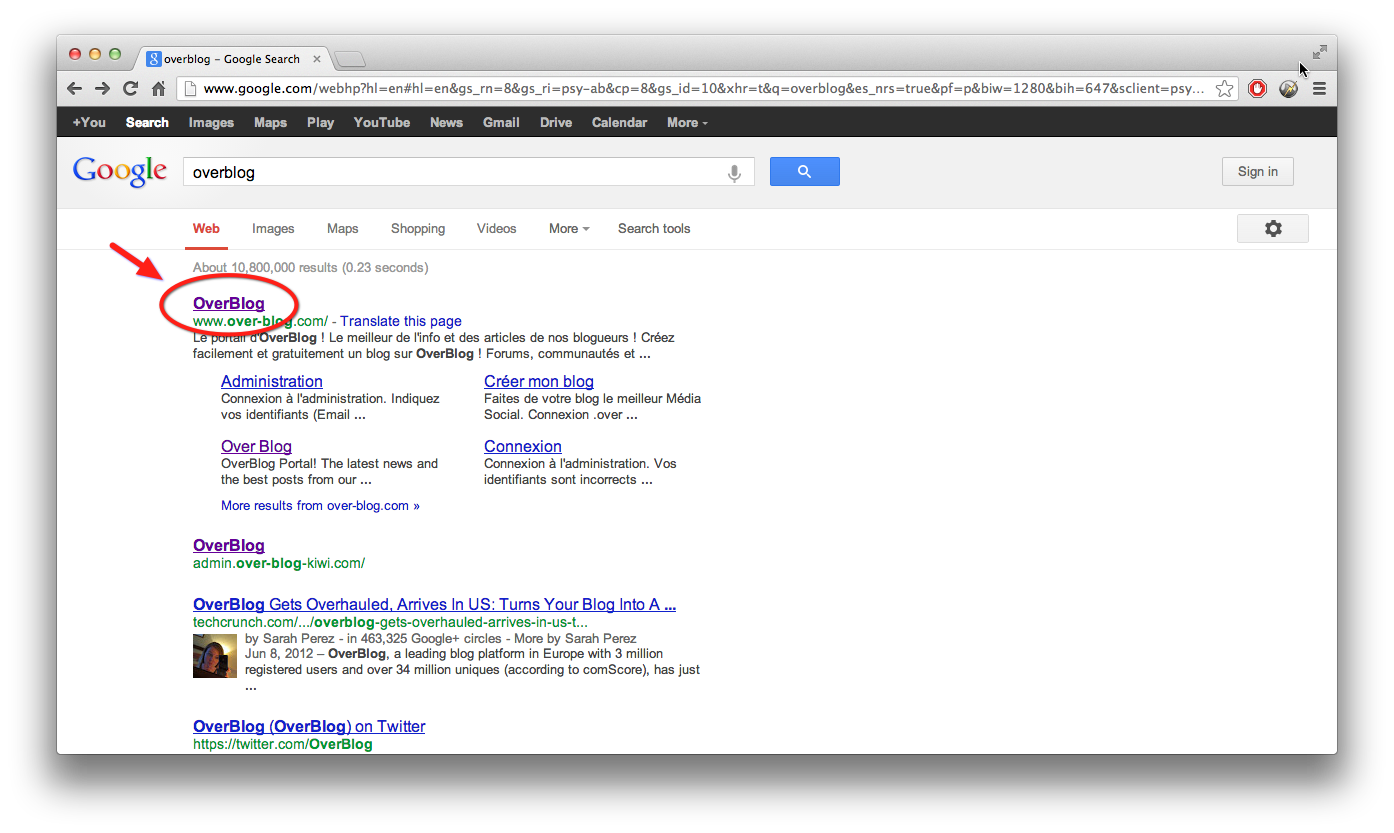
\includegraphics[width=13cm]{Images/linkOverblog.png}
    \caption{Overblog's link}
\end{figure}
Or you can also type in your adress bar this link \url{http://en.over-blog.com/}
\item Now, you have to sign up. Go at the end of the page and click on \emph{Sign up now} like this:
\begin{figure}[H]
    \center
	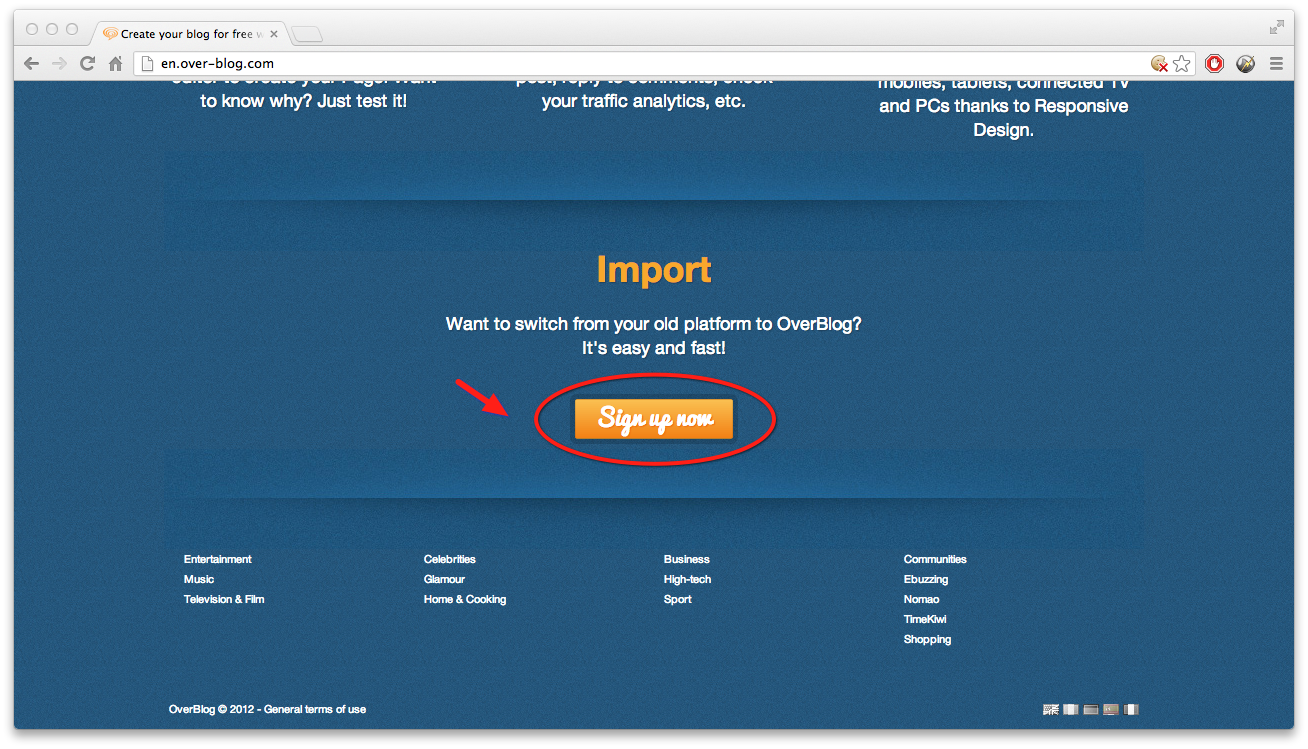
\includegraphics[width=13cm]{Images/signUpButton.png}
    \caption{Sign up button}
\end{figure}
\item Then you are redirected to this page:
\begin{figure}[H]
    \center
	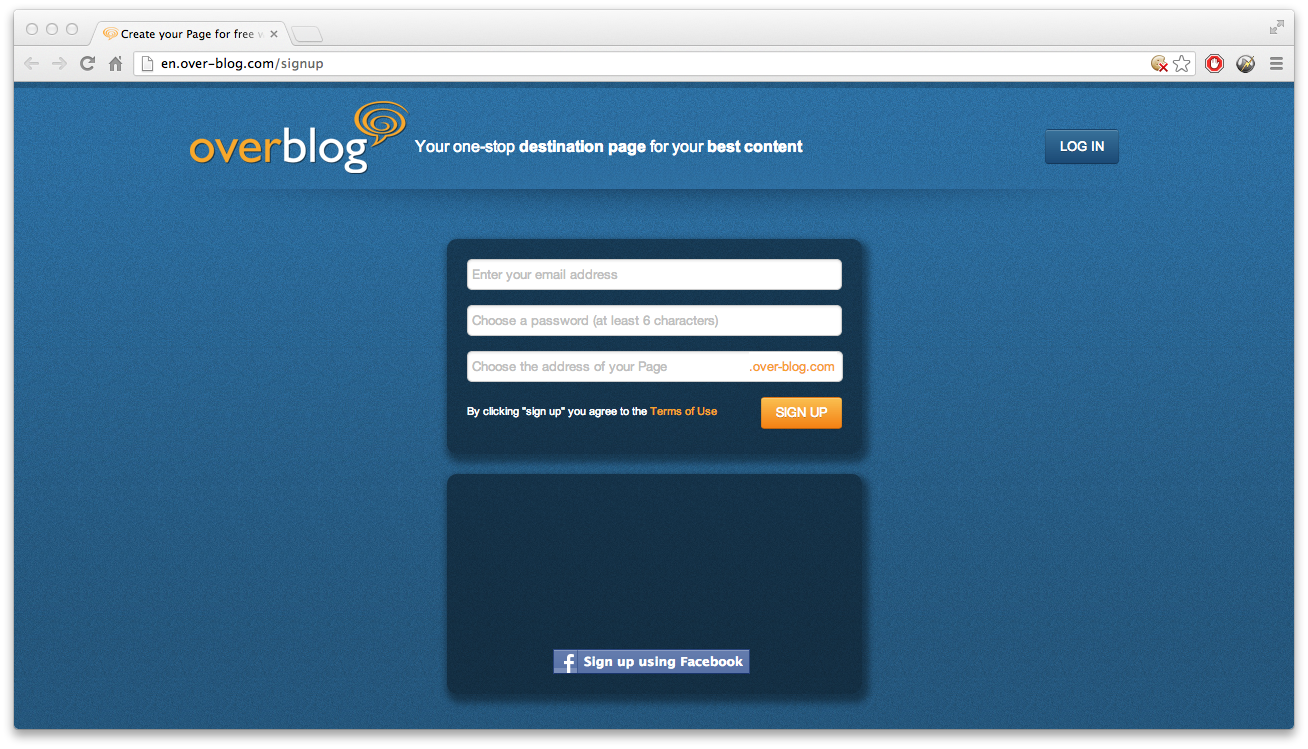
\includegraphics[width=13cm]{Images/signUpPage.png}
    \caption{Sign up page}
\end{figure}
You have to enter a valide email address because in the next step you have to confirm your registration by clicking a link wich is send on it. Moreover, you have to enter a password and the begining of your address you want for your blog (you have no choice for the end of the address, she must finish with \emph{.over-blog.com}. Here is an example:
\begin{figure}[H]
    \center
	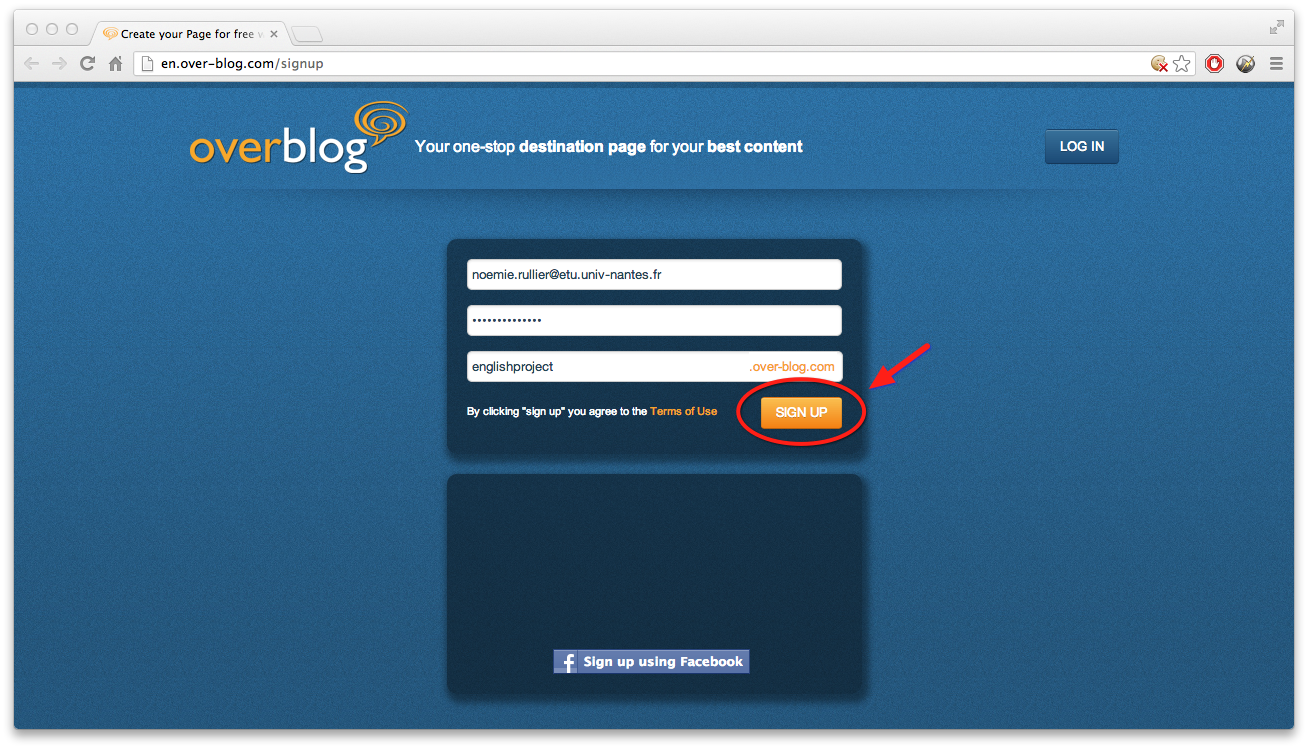
\includegraphics[width=13cm]{Images/signUpPageValues.png}
    \caption{Sign up page with values}
\end{figure}
Then click on \emph{SIGN UP}.
\item Then you are redirected on this page:
\begin{figure}[H]
    \center
	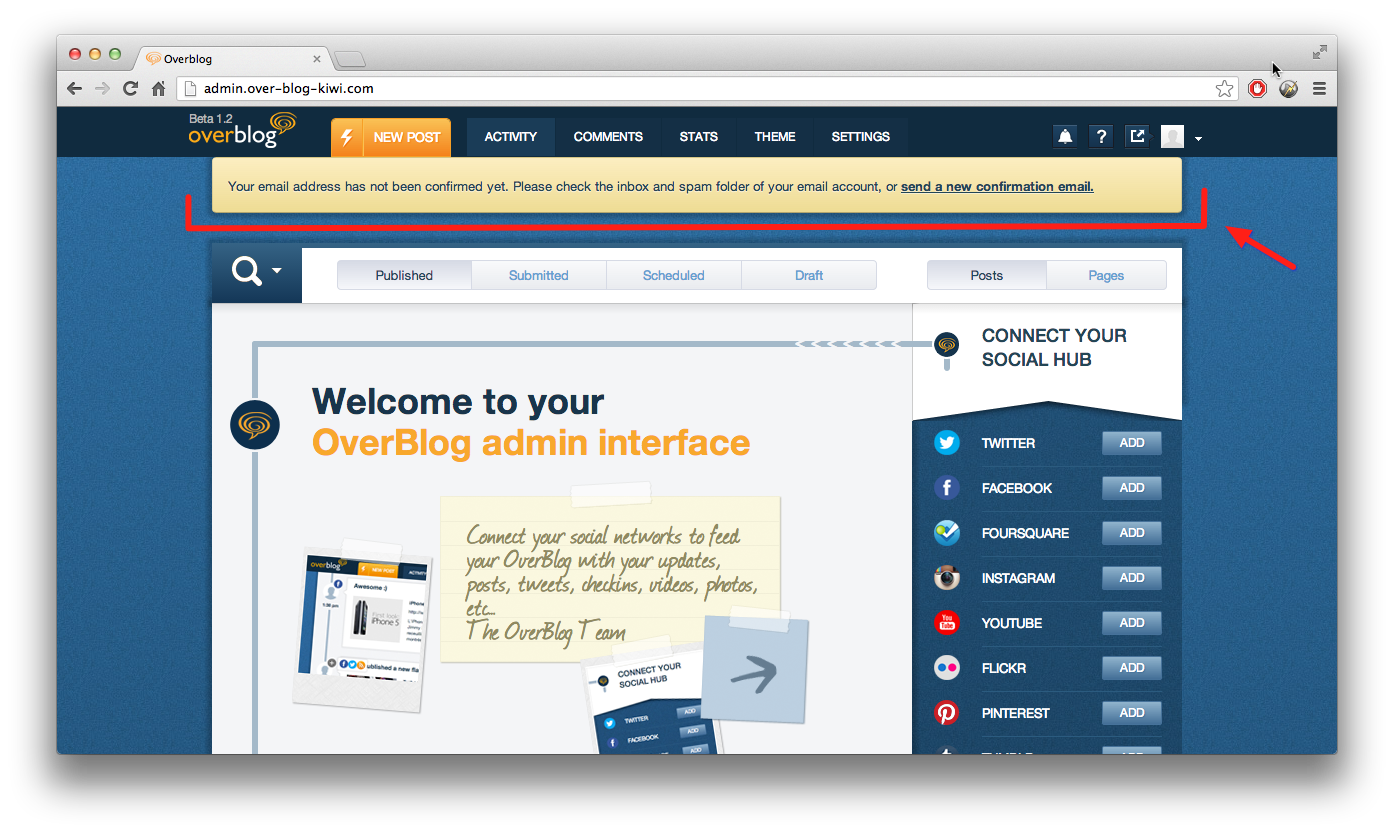
\includegraphics[width=13cm]{Images/addressMailNotConfirmed.png}
    \caption{Email address not confirmed}
\end{figure}
You can see that you have no confirmed you address email. Open your personal information manager, and open the mail send by \emph{marie@overblog.com}. If you don't see this mail, refresh your mail or look in your spam folder. The mail should look like that:
\begin{figure}[H]
    \center
	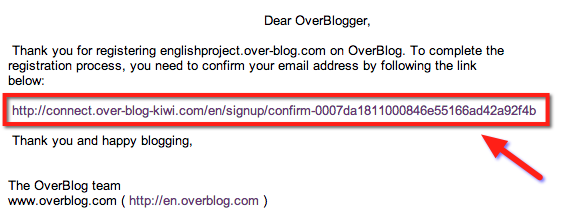
\includegraphics[width=10cm]{Images/emailOverblog.png}
    \caption{Email send by overblog}
\end{figure}
Click on the link surrounded in red. You are redirected on this page:
\begin{figure}[H]
    \center
	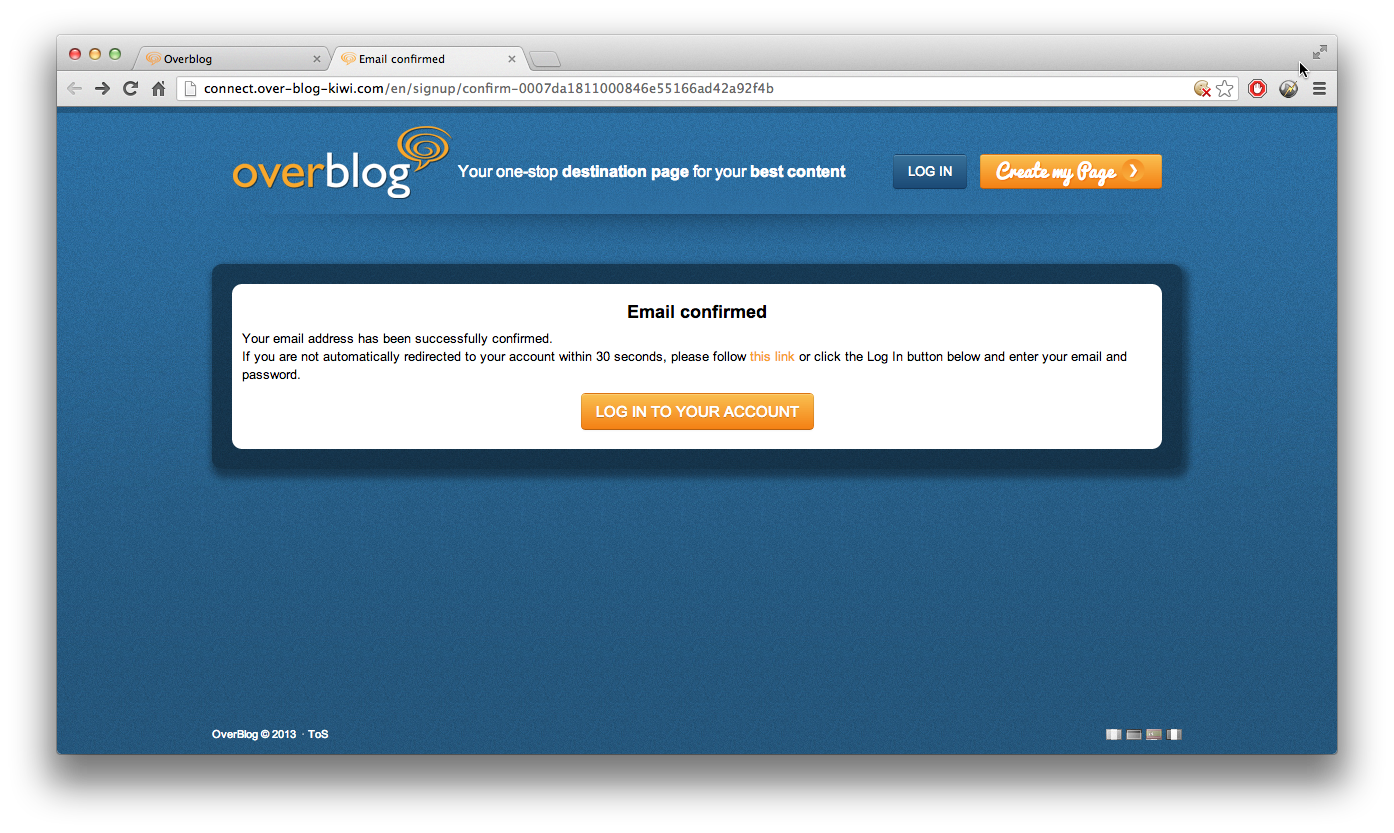
\includegraphics[width=13cm]{Images/addressMailConfirmed.png}
    \caption{Email address confirmed}
\end{figure}
To finish you are redirected on this page:
\begin{figure}[H]
    \center
	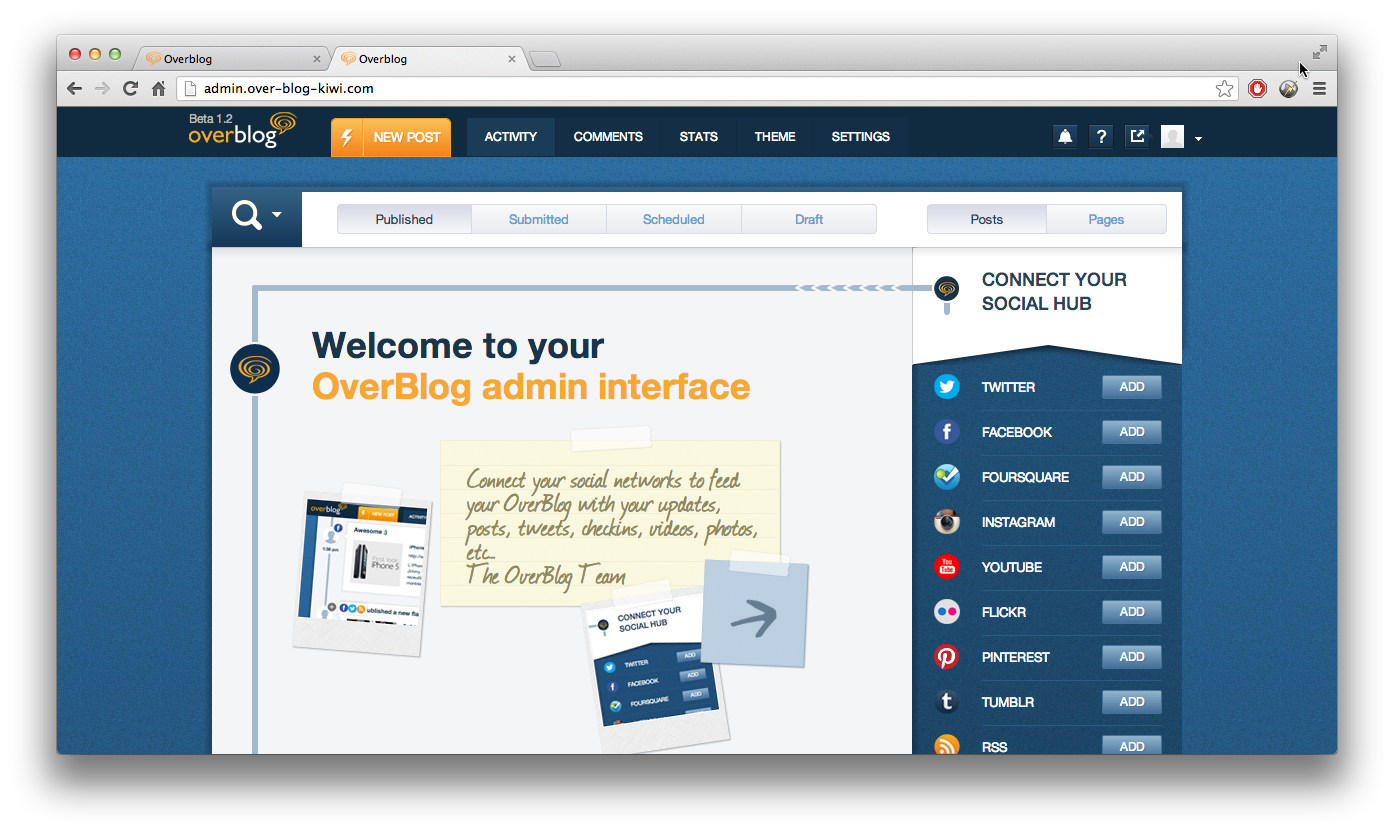
\includegraphics[width=13cm]{Images/overblogPage.png}
    \caption{Overblog's home page}
\end{figure}
Now you can start to enrich your blog !
\end{enumerate}


%%%%%%%%%%%%%%%%%%%%%%%%%%%%%%%%%%%%%%%%%%%%%%%%%%%%%%%%%%%%%%%%%%%%%%%%%%%%%
%%%%%%%%%%  Etape 2
%%%%%%%%%%%%%%%%%%%%%%%%%%%%%%%%%%%%%%%%%%%%%%%%%%%%%%%%%%%%%%%%%%%%%%%%%%%%%
\newpage
\section{Create an article}
%TODO Clément
%I - Texte
%II – Media (image/video/son)



%%%%%%%%%%%%%%%%%%%%%%%%%%%%%%%%%%%%%%%%%%%%%%%%%%%%%%%%%%%%%%%%%%%%%%%%%%%%%
%%%%%%%%%%  Etape 3
%%%%%%%%%%%%%%%%%%%%%%%%%%%%%%%%%%%%%%%%%%%%%%%%%%%%%%%%%%%%%%%%%%%%%%%%%%%%%
\newpage
\section{Personalise your blog}
%TODO Guillaume
% Fond d’écran / catégorie / résumé


%%%%%%%%%%%%%%%%%%%%%%%%%%%%%%%%%%%%%%%%%%%%%%%%%%%%%%%%%%%%%%%%%%%%%%%%%%%%%
%%%%%%%%%%  Etape 4
%%%%%%%%%%%%%%%%%%%%%%%%%%%%%%%%%%%%%%%%%%%%%%%%%%%%%%%%%%%%%%%%%%%%%%%%%%%%%
\newpage
\section{Sharing it}
%TODO Antoine
% Lien vers extérieur et partage réseaux sociaux (Antoine)

\subsection{Social linkage}

The first time you come to the  \emph{Overblog admin interface} you cannot miss this Panel.
\begin{figure}[h]
    \center
  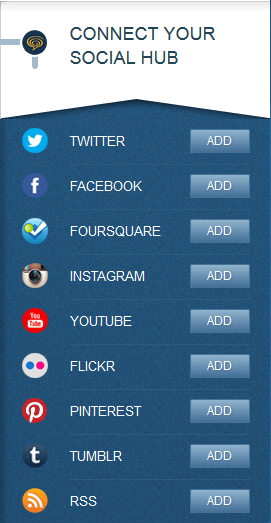
\includegraphics[width=0.3\textwidth]{Images/shareIni.png}
    \caption{Share panel}
\end{figure}

You can use it by clicking one of the button, like the facebook button (if you have a facebook account). Then agree with their proposal. With this linkage, you can feed your blog ! You are not obliged to rewrite your facebook publications.

In an other way, this linkage can allow your blog to ask your ``friends" to see your blog.

\subsection{Publish it on your favorites social networks !}

You can like your publications, or quote it by using the bar just under it.

\begin{figure}[h]
    \center
  
\includegraphics[width=0.9\textwidth]{Images/articleBar.png}
    \caption{Like bar}
\end{figure}

Your are also able to share your article, even your blog, on your favorite social network. You just need to click on one of the following buttons.

\begin{figure}[h]
    \center
  
\includegraphics[width=0.5\textwidth]{Images/blogBar.png}
    \caption{Share bar}
\end{figure}

\subsection{Purpose}

But why do all that ? To make your friends come to see your blog, comment it, like it, and share it with their own friends ! So more and more people can came to your blog and see your kiwi jam ! So let's do it.

 


%%%%%%%%%%%%%%%%%%%%%%%%%%%%%%%%%%%%%%%%%%%%%%%%%%%%%%%%%%%%%%%%%%%%%%%%%%%%%
%%%%%%%%%%  CONCLUSION GENERALE
%%%%%%%%%%%%%%%%%%%%%%%%%%%%%%%%%%%%%%%%%%%%%%%%%%%%%%%%%%%%%%%%%%%%%%%%%%%%%
\newpage
\section{Conclusion}
%TODO

\end{document}

\begin{figure}[H]
    \center
    \subfloat[Boîte de dialogue pour le nom de la tâche]{\includegraphics[width=3.7cm]{Images/addTask.png}}\quad
    \subfloat[Tâche]{\includegraphics[width=3.7cm]{Images/listTask.png}}
    \caption{Ajout d'une tâche}
\end{figure}